\section{Analysis exploiting a fit to $W$ $m_T$ to get background normalizations}
\label{sec:UVaND}
% ---- ---- ---- ---- ---- ---- ---- ---- ---- ---- ---- ---- ---- ---- ---- ---- ---- ---- ---- ---- ---- ---- ----

\subsection{Extraction of the Normalization for $W+$jets and QCD Multijet Production}\label{sec:UVaND_MTfits}



The sidebands of the Mjj distribution are a valuable source of
information that can be used to estimate the normalization in our
selected signal region for two difficult to model backgrounds: W+jets
and QCD.

The transverse mass of the leptonically decaying W can be used to
discriminate between W+jets and QCD, since W+jets contains a real W
whereas QCD does not. For this reason we fit the $M_T$ distribution in
the Mjj sidebands of the data, using the background shapes from MC, to
extract the normalizations of these processes. To fully exploit the
discriminating power of the $M_T$ shapes we chose to use the full
distribution and so remove the $M_T$ cut with respect to our event
selection described in Section~\ref{sec:firstStep}. We also relax the
MET requirement in the event selection to $25\,\mathrm{GeV}$ to
improve the statistics in the selected QCD sample.

From this selected data sample we construct the $M_T$ distribution and
subtract the other major backgrounds (whose normalizations are small
or reasonably well-known): $WW$, $WZ$, $Z$+jets, $t\bar{t}$, and
single-$t$. We extract the normalizations of the remaining
backgrounds, $W$+jets and QCD, by performing a two-component fit to the
background-subtracted data.

To assess the reliability of such a technique and the size of any
bias, we perform MC-only pseudoexperiments. Pseudodata are constructed
using MC events from these two processes. Their normalizations are
determined from Poisson-fluctuations in the predicted yields from MC.
The pseudodata are then fit with the shapes from $W$+jets and QCD (see
Fig.~\ref{fig:UVaND_mu_mtrans_fits} for the shape comparison).  From
the pull distribution for the fitted $W$+jets component, shown in
Figure~\ref{fig:UVaND_mu_mtrans_fits_pulls}, we see that in these
MC-only PEs we introduce a small bias but that the uncertainty from
the fit is reasonable.

The result of the $M_T$ fit in data is shown in
Figure~\ref{fig:UVaND_mu_mtrans_fits}. We find a small increase in the
$W$+jets normalization with respect to MC is necessary, which we
report as a scale factor which is then applies to the normalisation in
our signal region.

This technique relies on the shape of the $M_T$ distribution from
$W$+jets MC. Sources of systematic uncertainty incurred using this
shape include: uncertainty in the Jet Energy Scale (JES) which affects
the MET; renormalization and factorization scale assumptions in the
$W$+jets MC; and parton-jet matching threshold assumptions in the
Madgraph ME+PS $W$+jets MC sample construction. We assess the impact
of these shape uncertainties individually in MC-only
pseudoexperiments, constructing the pseudodata using $M_T$ shapes from
the MC which include $\pm1\sigma$ fluctuations for each source of
uncertainty. This pseudodata is fit with the nominal $M_T$ templates
and the resulting bias is incorporated as a relative uncertainty on
the $W$+jets scale factor. An additional systematic uncertainty comes
from the imprecise knowledge of the normalizations of the backgrounds
we subtract from the sideband data. We assumed a conservative 30\%
relative uncertainty on the subtracted backgrounds and then repeated
the the $M_T$ fit using the nominal MC templates. The impact of each
of these systematic uncertainties is summarized in
Table~\ref{tab:UVaND_WjetsQCD_SF_systs}. We find a final scale factor
for $W$+jets of

\begin{equation}
1.025 \pm 0.003 \mathrm{(stat)} \pm 0.019 \mathrm{(sys)} = 1.025 \pm 0.020.
\end{equation}

We expect QCD to be a relatively small contribution in our selected
signal sample but as an additional result of the $M_T$ fit, we can
obtain a scale factor for this process as well. The sideband data
prefers less QCD than predicted by the MC. For this QCD scale factor
we incorporate the systematic uncertainty due to JES and uncertainty
in the normalizations in the subtracted backgrounds. The scale factor
for QCD is

\begin{equation}
0.568 \pm 0.076 \mathrm{(stat)} \pm 0.735 \mathrm{(sys)} = 0.568 \pm 0.739.
\end{equation}

In the $e$+jets channel, we perform a similar fit to extract the
$W$+jets normalization from data. Even with our relaxed selection, an
$M_T$ template, usable in the fit, for QCD was not possible to
construct due to the MC statistics. Therefore, in this channel, we
subtract QCD from the sideband data as we do for the other background
processes and we assume a 100\% uncertainty on its normalization. The
same systematic uncertainties are considered on the $W$+jets scale
factor as in the $\mu$+jets channel. We find a scale factor for
$W$+jets in the electron channel of

\begin{equation}
1.018 \pm 0.003 \mathrm{(stat)} \pm 0.060 \mathrm{(sys)} = 1.018 \pm 0.060.
\end{equation}

The systematic uncertainties on the $W$+jets scale factors in both
channels are summarized in Table~\ref{tab:UVaND_WjetsQCD_SF_systs}.


\begin{figure}[h!]
\caption{Pseudoexperiment tests of the $W$+jets and QCD normalization
extraction technique in the $\mu+$jets channel.}\label{fig:UVaND_mu_mtrans_fits_pulls}
\begin{center}$
\begin{array}{c}
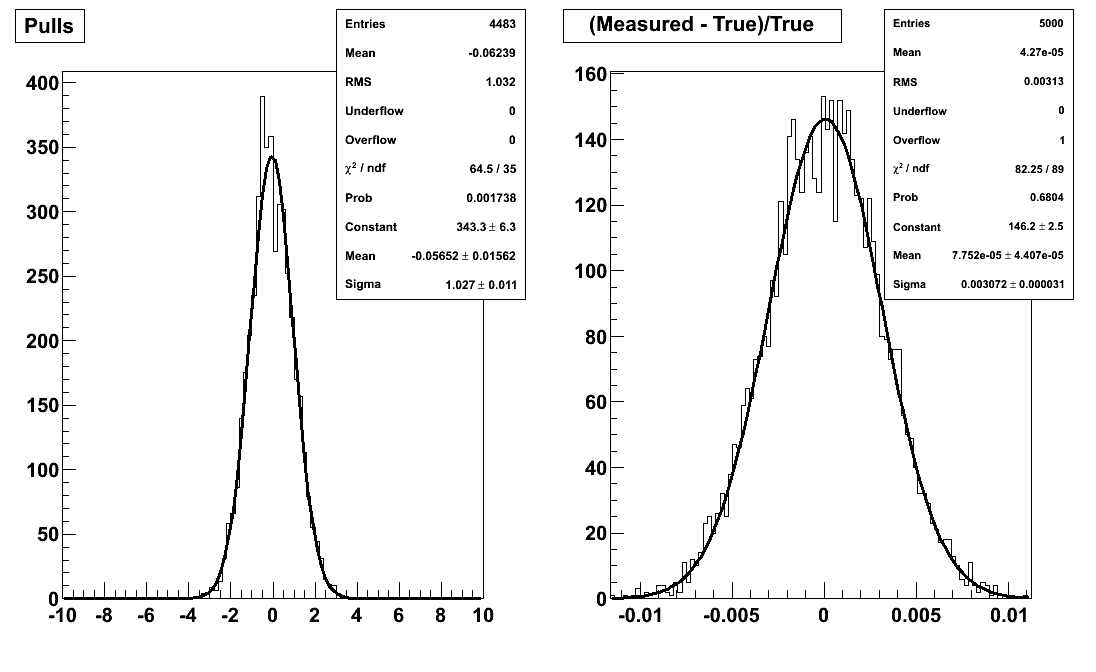
\includegraphics[width=6in]{plots/mu_xsWJets_PullMeas.png}
\end{array}$
\end{center}
\end{figure}


\begin{figure}[h!]
\caption{Shape comparison
of the the $W+jets$ and QCD $M_T$ distributions (left),
the comparison of the summed MC prediction for $W$+jets and QCD
to the other-background-subtracted sideband data before the fit (center) and
the resulting comparison after the fit, incorporating the new normalization 
of these background components (right).}\label{fig:UVaND_mu_mtrans_fits}
\begin{center}$
\begin{array}{ccc}
\hspace{-0.5in}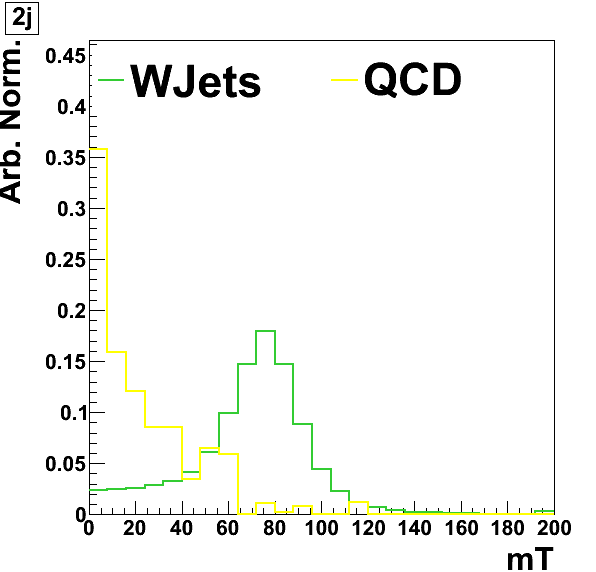
\includegraphics[width=2.5in]{plots/mu_templates_mT.png} &
\hspace{-0.25in}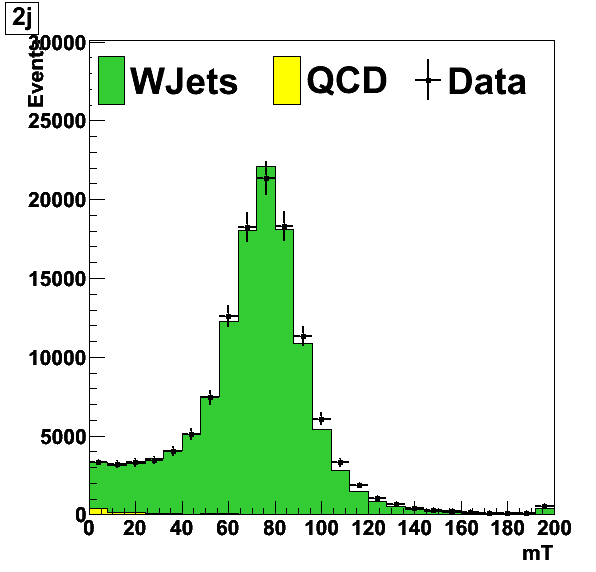
\includegraphics[width=2.5in]{plots/mu_stack_mT_beforeFit.png} &
\hspace{-0.25in}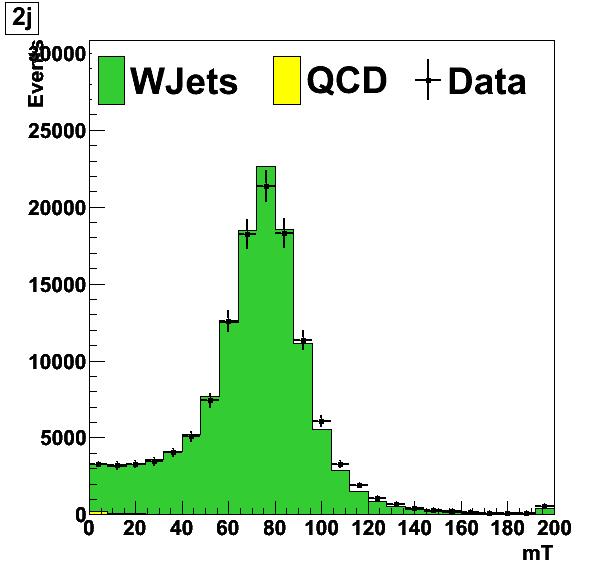
\includegraphics[width=2.5in]{plots/mu_stack_mT_afterFit.png}
\end{array}$
\end{center}
\end{figure}

\begin{table}[h!]
\centering
\caption{Effect of systematic uncertainties on the $W+$jets scale
factors in the $\mu$ and $e+$ jets channels. Values are reported raw,
not relative, with respect to the actual central
values.}\label{tab:UVaND_WjetsQCD_SF_systs}
\begin{tabular}{ccc} \hline
Source & $e+$jets & $\mu+$jets \\ \hline
JES    & $\pm 0.0073$     & $\pm 0.0074$      \\
$Q^2$  & $\pm 0.0155$     & $\pm 0.0070$      \\
matching & $\pm 0.0137$     & $\pm 0.0062$      \\
bkg subtraction & $\pm 0.0563$    & $\pm 0.0152$     \\ \hline
Total  & $\pm 0.0601$ & $\pm 0.0193$   \\ \hline
\end{tabular}
\end{table}

\clearpage
\subsection{Extraction of signal limits}

Limits are calculated using the standard Higgs group limit setting
machinery~\cite{HiggsCombine}.  For the moment the expected limits are
computed using the {\it ProfileLikelihood} method, but for the final
results, the standard CLs limit calculation technique will be
employed.  Expected limits are calculated using 3000
pseudo-experiments.  Limits are calculated separately for the muon +
jets and the electron + jets channel, as well as for the sum of the
two channels.  The limits are calculated using two different
approaches:

\subsubsection{Signal Limit Extraction in Counting Experiments in Windows of $M_{\ell \nu jj}$}
These limits are based on a simple ``cut and count'' approach.  After
the event selection described above, a window cut is applied in the
$\ell\nu jj$ invariant mass $M_{\ell\nu jj}$ distribution and a limit
is extracted by comparing the background prediction in that window to
the ``observed'' events in pseudodata.  The actual $M_{\ell\nu jj}$
window used varies with the Higgs mass hypothesis being tested. The
yields in these windows for background and signal for the $\mu$+jets
channel are described in Tables~\ref{tab:muonBKGwindows} and
\ref{tab:muonSIGwindows} and for the $e$+jets channel in
Tables~\ref{tab:electronBKGwindows} and \ref{tab:electronSIGwindows}.

The expected 95\% C.L. limits obtained with this
procedure are detailed in Tables~\ref{tab:CutAndCount} and \ref{tab:CutAndCount_ele} and represented
graphically in Fig.~\ref{fig:CutAndCount} and \ref{fig:CutAndCount_ele}.

%BACKGROUND MUON
\clearpage
\begin{table}
\begin{adjustwidth}{-1.7in}{-1.7in} 
  \centering 
    \begin{tabular}{|l|c|c|c|c|c|c|c|c|c|} \hline 
Cut & $WW$ & $WZ$ & $W$+jets & $Z$+jets & $t\bar{t}$ & $t$ & QCD & Sum Bkg & Data \\ \hline 
Total & 644.67 & 115.29 & 24822.04 & 692.99 & 448.07 & 212.27 & 39.86 & 26883.50 & 25505.00 \\ \hline 
225$<$Mlvjj$<$275 & 135.98 & 27.59 & 5259.86 & 155.83 & 105.32 & 55.75 & 0.00 & 5740.33 & 5611.00 \\ \hline 
270$<$Mlvjj$<$330 & 93.96 & 19.92 & 3148.99 & 92.65 & 112.47 & 45.94 & 0.00 & 3513.93 & 3694.00 \\ \hline 
310$<$Mlvjj$<$390 & 76.20 & 15.83 & 2252.86 & 55.93 & 97.18 & 36.22 & 0.00 & 2534.22 & 2651.00 \\ \hline 
355$<$Mlvjj$<$445 & 53.01 & 10.34 & 1366.70 & 30.06 & 73.19 & 25.54 & 0.00 & 1558.85 & 1726.00 \\ \hline 
390$<$Mlvjj$<$510 & 46.01 & 8.49 & 1070.45 & 24.92 & 64.09 & 21.43 & 0.00 & 1235.39 & 1437.00 \\ \hline 
415$<$Mlvjj$<$575 & 42.19 & 7.22 & 905.28 & 20.96 & 54.67 & 19.09 & 0.00 & 1049.40 & 1251.00 \\ \hline 
470$<$Mlvjj$<$610 & 24.28 & 3.93 & 512.65 & 8.04 & 27.38 & 9.27 & 0.00 & 585.56 & 631.00 \\ \hline 
485$<$Mlvjj$<$665 & 23.39 & 3.71 & 451.09 & 7.44 & 26.73 & 8.74 & 0.00 & 521.10 & 590.00 \\ \hline 
     \end{tabular} 
  \end{adjustwidth} 
    \caption{Expected background yields in 2.084~fb$^{-1}$ and data
    yields in the muon channel in chosen M(l$\nu$jj) windows. The
    background yields are taken from MC except for W+jets and QCD
    whose yields are taken from MC scaled by the scale factor found in
    Section~\ref{sec:UVaND_MTfits}}.
    \label{tab:muonBKGwindows} 
\end{table} 

%SIGNAL MUON

\begin{table} 
  \centering 
    \begin{tabular}{|l|c|c||c|c|c|} \hline 
$M_{H}$ & Yield & $S/\sqrt{B}$ & Mlvjj window cuts & Yield & $S/\sqrt{B}$ \\ \hline
250 & 61.51 & 0.38 & 225$<$Mlvjj$<$275 & 42.10 & 0.56 \\ \hline 
300 & 56.58 & 0.35 & 270$<$Mlvjj$<$330 & 38.68 & 0.65 \\ \hline 
350 & 64.00 & 0.39 & 310$<$Mlvjj$<$390 & 46.01 & 0.92 \\ \hline 
400 & 53.77 & 0.33 & 355$<$Mlvjj$<$445 & 36.13 & 0.92 \\ \hline
450 & 36.78 & 0.22 & 390$<$Mlvjj$<$510 & 25.94 & 0.74 \\ \hline 
500 & 22.14 & 0.14 & 415$<$Mlvjj$<$575 & 16.35 & 0.50 \\ \hline 
550 & 13.83 & 0.08 & 470$<$Mlvjj$<$610 & 8.98 & 0.37 \\ \hline 
600 & 8.24 & 0.05 & 485$<$Mlvjj$<$665 & 5.53 & 0.24 \\ \hline 
    \end{tabular} 
    \caption{Expected signal MC yields in 2.084fb~$^{-1}$ in the muon
    channel and the $S/\sqrt{B}$ values for each $M_{H}$ for the total
    M(l$\nu$jj) sample (left) and in the given M(l$/nu$jj) window
    (right).}
    \label{tab:muonSIGwindows} 
\end{table} 


%BACKGROUND ELECTRON
\clearpage
\begin{table}
\begin{adjustwidth}{-1.7in}{-1.7in} 
  \centering 
    \begin{tabular}{|l|c|c|c|c|c|c|c|c|c|} \hline 
Cut & $WW$ & $WZ$ & $W$+jets & $Z$+jets & $t\bar{t}$ & $t$ & QCD & Sum Bkg & Data \\ \hline 
Total & 516.03 & 90.53 & 18393.43 & 350.46 & 374.14 & 167.48 & 321.97 & 20170.51 & 19339.00 \\ \hline 
225$<$Mlvjj$<$275 & 106.97 & 21.80 & 3971.66 & 93.29 & 86.12 & 44.15 & 0.00 & 4323.99 & 4298.00 \\ \hline
270$<$Mlvjj$<$330 & 80.51 & 15.32 & 2514.45 & 48.21 & 84.97 & 33.99 & 0.00 & 2777.46 & 2846.00 \\ \hline 
310$<$Mlvjj$<$390 & 65.61 & 12.30 & 1933.82 & 33.07 & 85.50 & 28.57 & 321.97 & 2480.85 & 2310.00 \\ \hline
355$<$Mlvjj$<$445 & 43.70 & 8.47 & 1166.87 & 15.23 & 61.69 & 19.77 & 258.14 & 1573.87 & 1622.00 \\ \hline
390$<$Mlvjj$<$510 & 38.93 & 7.89 & 931.33 & 12.30 & 51.00 & 18.40 & 0.00 & 1059.85 & 1293.00 \\ \hline
415$<$Mlvjj$<$575 & 37.63 & 7.09 & 882.90 & 9.53 & 49.65 & 17.42 & 0.00 & 1004.23 & 1127.00 \\ \hline 
470$<$Mlvjj$<$610 & 23.20 & 4.26 & 496.24 & 5.00 & 28.18 & 8.99 & 0.00 & 565.87 & 580.00 \\ \hline 
485$<$Mlvjj$<$665 & 23.73 & 4.14 & 469.53 & 5.59 & 25.06 & 8.83 & 0.00 & 536.88 & 575.00 \\ \hline 
    \end{tabular} 
  \end{adjustwidth} 
    \caption{Expected background yields in 2.084~fb$^{-1}$ and data
    yields in the electron channel in chosen M(l$\nu$jj) windows. The
    background yields are taken from MC except for W+jets whose yields
    are taken from MC scaled by the scale factor found in
    Section~\ref{sec:UVaND_MTfits}}.
    \label{tab:electronBKGwindows} 
\end{table} 

\begin{table} 
  \centering
    \begin{tabular}{|l|c|c||c|c|c|} \hline 
$M_{H}$ & Yield & $S/\sqrt{B}$ & Mlvjj window cuts & Yield & $S/\sqrt{B}$ \\ \hline
250 & 49.71 & 0.35 & 225$<$Mlvjj$<$275 & 35.10 & 0.53 \\ \hline
300 & 50.10 & 0.35 & 270$<$Mlvjj$<$330 & 34.51 & 0.65 \\ \hline 
350 & 58.03 & 0.41 & 310$<$Mlvjj$<$390 & 41.70 & 0.84 \\ \hline
400 & 49.94 & 0.35 & 355$<$Mlvjj$<$445 & 33.46 & 0.84 \\ \hline
450 & 34.05 & 0.24 & 390$<$Mlvjj$<$510 & 24.62 & 0.76 \\ \hline
500 & 20.09 & 0.14 & 415$<$Mlvjj$<$575 & 15.09 & 0.48 \\ \hline 
550 & 12.97 & 0.09 & 470$<$Mlvjj$<$610 & 8.47 & 0.36 \\ \hline 
600 & 7.99 & 0.06 & 485$<$Mlvjj$<$665 & 5.49 & 0.24 \\ \hline
    \end{tabular} 
    \caption{Expected signal MC yields in 2.084~fb$^{-1}$ in the
    electron channel and the $S/\sqrt{B}$ values for each $M_{H}$ for
    the total M(l$\nu$jj) sample (left) and in the given M(l$/nu$jj)
    window (right).}
    \label{tab:electronSIGwindows} 
\end{table} 


\begin{table}[htdp]
\caption{Expected 95\% C.L. upper limits, as well as the 68\% and 95\%
bands on the expectation, on Higgs production quoted as a ratio to the
expected rate in the SM in the $\mu$+jets channel simple counting experiment.}
\begin{center}
\begin{tabular}{|c|c|c|c|c|c|}
\hline\hline
          &       & \multicolumn{2}{|c|}{68\% Range} & \multicolumn{2}{|c|}{95\% Range} \\
Mass & Median Exp. & Low & High & Low & High \\
\hline\hline
250  & 6.94  & 4.12 & 10.73 & 2.75 & 14.73 \\
300  & 5.03 & 3.09 & 7.85 & 2.09 & 10.58 \\
350  & 3.38 & 1.98 & 5.16  & 1.37 & 7.07 \\
400  & 2.92 & 1.77 & 4.59 & 1.18 & 6.25 \\
450  & 3.54 & 2.17 & 5.50 & 1.44 & 7.62 \\
500  & 5.09 & 3.07 & 7.95  & 2.06 & 10.76 \\
550  & 6.36 & 3.79 & 10.16 & 2.56 & 13.69 \\
600  & 9.83 & 5.99 & 15.22  & 4.03 & 21.02 \\
\hline\hline
\end{tabular}
\end{center}
\label{tab:CutAndCount}
\end{table}%

\begin{table}[htdp]
\caption{Expected 95\% C.L. upper limits, as well as the 68\% and 95\%
bands on the expectation, on Higgs production quoted as a ratio to the
expected rate in the SM in the $e$+jets channel simple counting experiment.}
\begin{center}
\begin{tabular}{|c|c|c|c|c|c|}
\hline\hline
          &       & \multicolumn{2}{|c|}{68\% Range} & \multicolumn{2}{|c|}{95\% Range} \\
Mass & Median Exp. & Low & High & Low & High \\
\hline\hline
250 &  13.89 & 8.19 & 22.06 & 5.20 & 30.59 \\
300 &  9.27 & 5.38  & 14.60 & 3.50 & 19.77 \\
350 &  11.56  & 4.83 & 20.85 & 3.01 & 39.59 \\
400 &  10.40 & 4.20 & 19.17 & 2.37 & 36.59 \\
450 &  5.44 & 3.16 & 8.42 & 2.02 & 11.46 \\
500 &  8.36 & 4.90  & 13.13 & 3.15 & 18.16 \\
550 &  9.22 & 5.44 & 14.61 & 3.66 & 20.48 \\
600 &  13.94 & 8.13  & 21.92 & 5.31 & 29.97 \\
\hline\hline
\end{tabular}
\end{center}
\label{tab:CutAndCount_ele}
\end{table}%

%\begin{table}[htdp]
%\caption{Expected 95\% C.L. upper limits, as well as the 68\% and 95\%
%bands on the expectation, on Higgs production quoted as a ratio to the
%expected rate in the SM in the combined $\mu$ and $e$+jets channel simple counting experiment.}
%\begin{center}
%\begin{tabular}{|c|c|c|c|c|c|}
%\hline\hline
%          &       & \multicolumn{2}{|c|}{68\% Range} & \multicolumn{2}{|c|}{95\% Range} \\
%Mass & Median Exp. & Low & High & Low & High \\
%\hline\hline
%300 &  6.43 & 3.81 & 9.89 & 2.54 & 13.58 \\
%350 &  6.60 & 3.10 & 11.25 & 1.92 & 20.59 \\
%400 &  5.96 & 2.56 & 10.85 & 1.59 & 19.33  \\
%450 &  3.89 & 2.33 & 6.09  & 1.54 & 8.37 \\
%500 &  5.79 & 3.40 & 9.05 & 2.25 & 12.42  \\
%550 &  6.42 & 3.90 & 9.88 & 2.63 & 13.39 \\
%600 &  9.72 & 5.71 & 14.96 & 3.83 & 20.62 \\
%\hline\hline
%\end{tabular}
%\end{center}
%\label{tab:CutAndCount_comb}
%\end{table}%




\begin{figure}[htbp] %  figure placement: here, top, bottom, or page
   \centering
   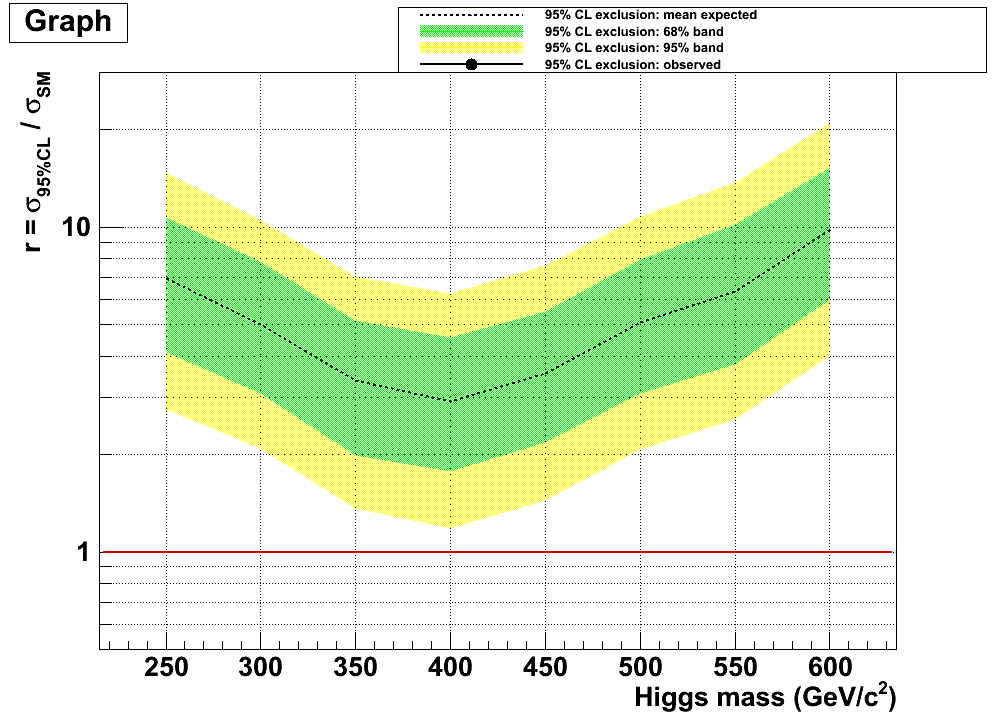
\includegraphics[width=4in]{plots/UVaND_muon_sc.png} 
   \caption{Observed and expected 95\% C.L. upper limits, as well as
   the 68\% and 95\% bands on the expectation, on Higgs production
   quoted as a ratio to the expected rate in the SM in the $\mu$+jets channel simple counting experiment.}
   \label{fig:CutAndCount}
\end{figure}

\begin{figure}[htbp] %  figure placement: here, top, bottom, or page
   \centering
   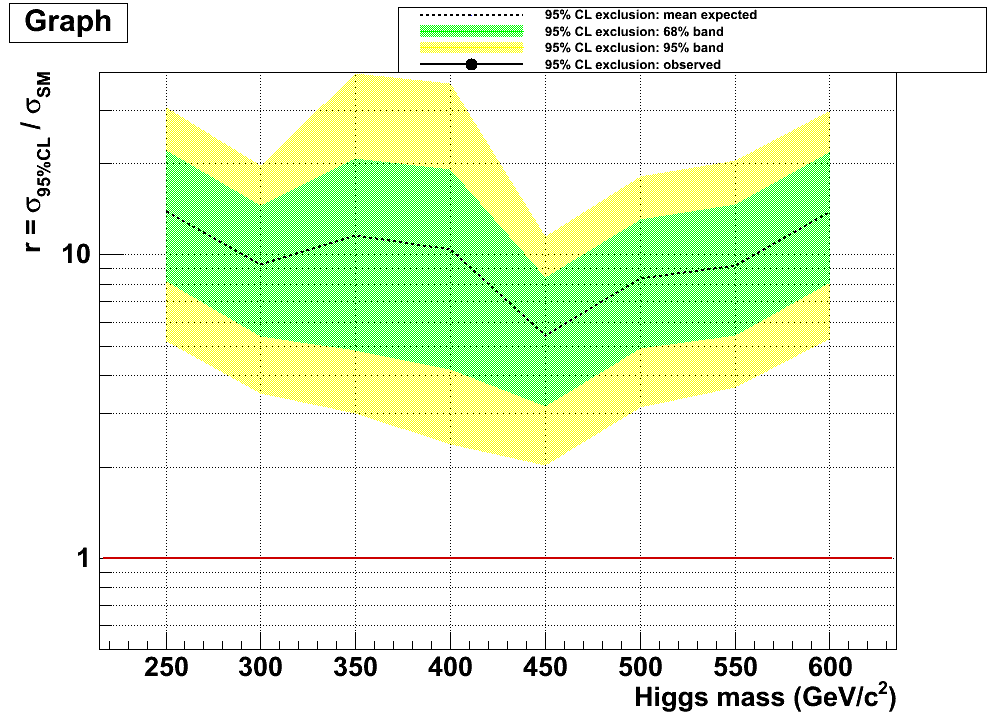
\includegraphics[width=4in]{plots/UVaND_ele_sc.png} 
   \caption{Observed and expected 95\% C.L. upper limits, as well as
   the 68\% and 95\% bands on the expectation, on Higgs production
   quoted as a ratio to the expected rate in the SM in the $e$+jets channel simple counting experiment.}
   \label{fig:CutAndCount_ele}
\end{figure}

%\begin{figure}[htbp] %  figure placement: here, top, bottom, or page
%   \centering
%   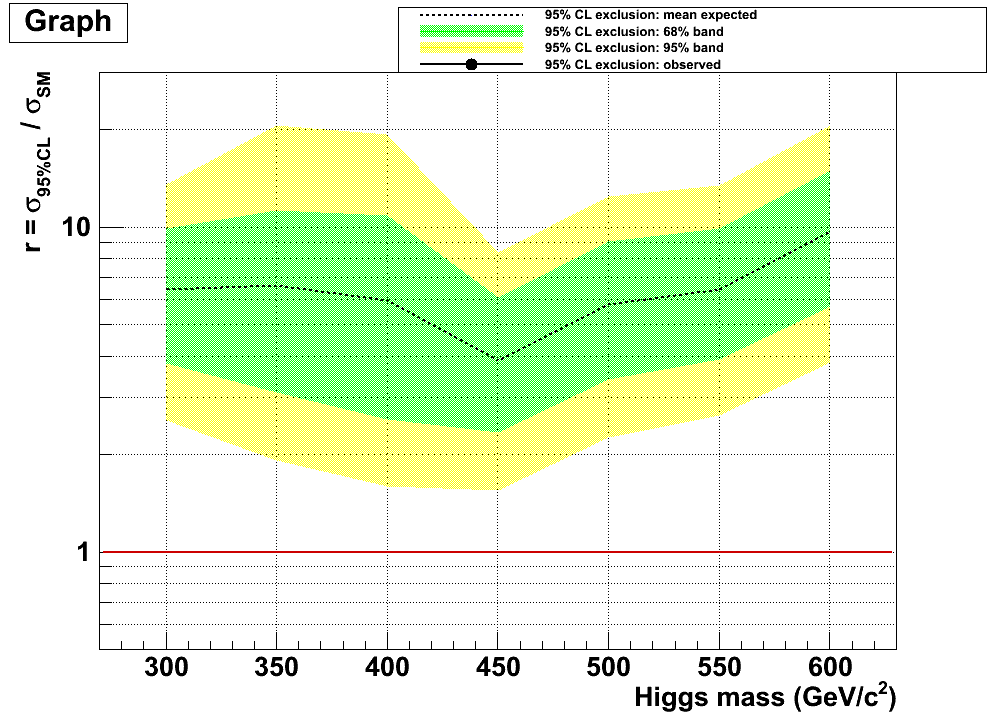
\includegraphics[width=4in]{plots/UVaND_combined_sc.png} 
%   \caption{Observed and expected 95\% C.L. upper limits, as well as
%   the 68\% and 95\% bands on the expectation, on Higgs production
%   quoted as a ratio to the expected rate in the SM in the combined $\mu$ and $e$+jets channel simple counting experiment.}
%   \label{fig:CutAndCount_comb}
%\end{figure}



\clearpage
\subsubsection{Signal Limit Extraction Using Full $M_{\ell \nu jj}$ Shape}
These limits are based on fitting the full $M_{\ell\nu jj}$
distribution. The yields in the full $M_{\ell\nu jj}$ distribution for
background and signal for the $\mu$+jets channel are also given in
Tables~\ref{tab:muonBKGwindows} and \ref{tab:muonSIGwindows} and for
the $e$+jets channel in Tables~\ref{tab:electronBKGwindows} and
\ref{tab:electronSIGwindows}.

In addition to accounting for the rate uncertainties in
the background, shape uncertainties associated with the jet energy
scale, and the Monte Carlo scale and matching uncertainties for the
$W$+jets, $Z$+jets, and $t\bar{t}$ samples are also included.

The expected 95\% C.L. limits obtained with this
procedure are detailed in Tables~\ref{tab:ShapeFit}, \ref{tab:ShapeFit_ele} and \ref{tab:ShapeFit_comb} and represented
graphically in Fig.~\ref{fig:ShapeFit}, \ref{fig:ShapeFit_ele} and \ref{fig:ShapeFit_comb}.

\begin{table}[htdp]
\caption{Expected 95\% C.L. upper limits, as well as the
68\% and 95\% bands on the expectation, on Higgs production quoted as
a ratio to the expected rate in the SM in the $\mu$+jets channel full $M_{\ell \nu jj}$ fits.}
\begin{center}
\begin{tabular}{|c|c|c|c|c|c|}
\hline\hline
          &           & \multicolumn{2}{|c|}{68\% Range} & \multicolumn{2}{|c|}{95\% Range} \\
Mass & Median Exp. & Low & High & Low & High \\
\hline\hline
250  & 4.28 & 0.92  & 9.87 & 0.60 & 15.61 \\
300  & 4.62 & 1.57  & 10.98 & 0.76  & 35.06 \\
350  & 2.38 & 0.49 & 7.58 & 0.29 & 21.12 \\
400  & 2.14 & 0.42  & 7.92  & 0.24 & 22.32 \\
450  & 2.21 & 0.51  & 5.99 & 0.30  & 25.26 \\
500  & 3.29 & 1.36   & 8.25 & 0.66 & 30.83 \\
550  & 4.75 & 2.23  & 9.53 & 1.14  & 28.56 \\
600  & 6.26 & 3.11  & 13.89 & 1.68  & 32.86 \\
\hline\hline
\end{tabular}
\end{center}
\label{tab:ShapeFit}
\end{table}%

\begin{table}[htdp]
\caption{Expected 95\% C.L. upper limits, as well as the
68\% and 95\% bands on the expectation, on Higgs production quoted as
a ratio to the expected rate in the SM in the $e$+jets channel full $M_{\ell \nu jj}$ fits.}
\begin{center}
\begin{tabular}{|c|c|c|c|c|c|}
\hline\hline
          &           & \multicolumn{2}{|c|}{68\% Range} & \multicolumn{2}{|c|}{95\% Range} \\
Mass & Median Exp. & Low & High & Low & High \\
\hline\hline
250  & 9.41 & 4.78 & 18.62 & 3.06 & 57.27 \\
300  & 6.89 & 3.50 & 12.78 & 2.22 & 33.90 \\
350  & 4.41 & 2.27 & 7.91 & 1.50 & 17.67 \\
400  & 3.14 & 1.64 & 5.80 & 0.98  & 12.10 \\
450  & 3.56 & 1.79 & 6.00 & 1.03  & 10.35 \\
500  & 4.16 & 2.27 & 7.27 & 1.31 & 11.86 \\
550  & 4.88   & 2.65 & 8.58 & 1.45 & 13.18 \\
600  & 6.85  & 3.68  & 11.67 & 2.08 & 17.81 \\
\hline\hline
\end{tabular}
\end{center}
\label{tab:ShapeFit_ele}
\end{table}%

\begin{table}[htdp]
\caption{Expected 95\% C.L. upper limits, as well as the
68\% and 95\% bands on the expectation, on Higgs production quoted as
a ratio to the expected rate in the SM in the combined $\mu$ and $e$+jets channel full $M_{\ell \nu jj}$ fits.}
\begin{center}
\begin{tabular}{|c|c|c|c|c|c|}
\hline\hline
          &           & \multicolumn{2}{|c|}{68\% Range} & \multicolumn{2}{|c|}{95\% Range} \\
Mass & Median Exp. & Low & High & Low & High \\
\hline\hline
250  & 5.47 & 3.03  & 8.44 & 1.97  & 12.98 \\
300  & 3.73 & 2.18  & 6.30 & 1.46  & 10.63  \\
350  & 2.42 & 1.46  & 4.25 & 0.98  & 6.35 \\
400  & 2.03 & 1.17  & 3.68 & 0.78  & 6.04 \\
450  & 2.30 & 1.29  & 3.84 & 0.84  & 5.68 \\
500  & 2.96 & 1.73  & 5.08 & 1.13  & 7.58 \\
550  & 3.60 & 2.08  & 6.21 & 1.29  & 9.05 \\
600  & 5.04 & 2.92  & 8.67 & 1.83  & 12.56 \\
\hline\hline
\end{tabular}
\end{center}
\label{tab:ShapeFit_comb}
\end{table}%

\begin{figure}[htbp] %  figure placement: here, top, bottom, or page
   \centering
   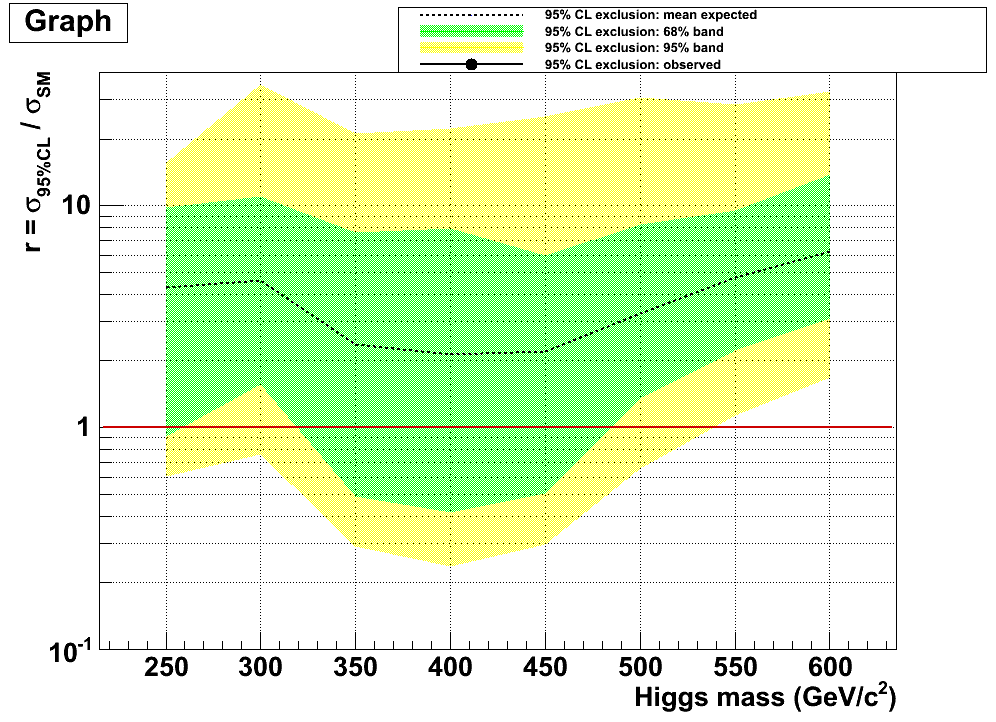
\includegraphics[width=4in]{plots/UVaND_muon.png} 
   \caption{Expected 95\% C.L. upper limits, as well as
   the 68\% and 95\% bands on the expectation, on Higgs production
   quoted as a ratio to the expected rate in the SM in the $\mu$+jets channel full $M_{\ell \nu jj}$ fits.}
   \label{fig:ShapeFit}
\end{figure}


\begin{figure}[htbp] %  figure placement: here, top, bottom, or page
   \centering
   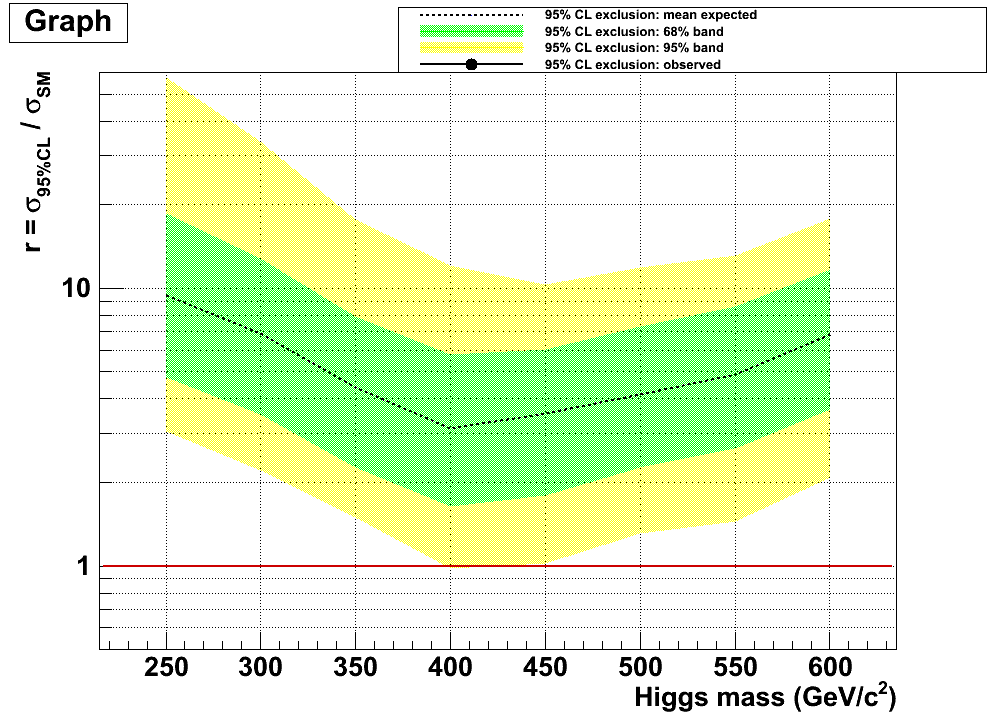
\includegraphics[width=4in]{plots/UVaND_ele.png} 
   \caption{Expected 95\% C.L. upper limits, as well as
   the 68\% and 95\% bands on the expectation, on Higgs production
   quoted as a ratio to the expected rate in the SM in the $e$+jets channel full $M_{\ell \nu jj}$ fits.}
   \label{fig:ShapeFit_ele}
\end{figure}


\begin{figure}[htbp] %  figure placement: here, top, bottom, or page
   \centering
   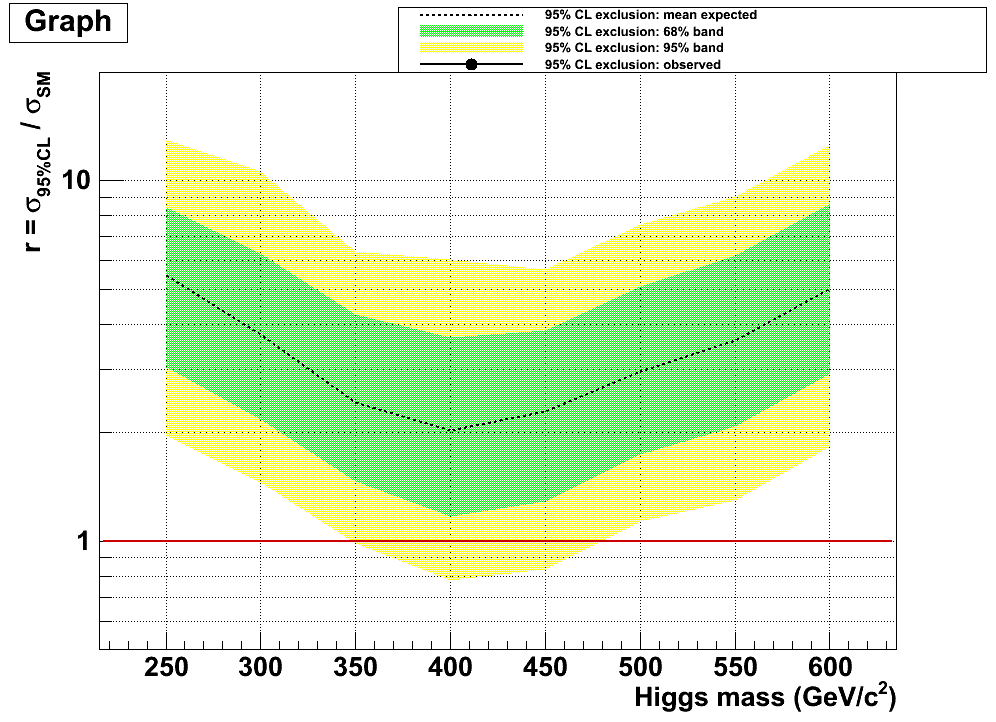
\includegraphics[width=4in]{plots/UVaND_combined.png} 
   \caption{Expected 95\% C.L. upper limits, as well as
   the 68\% and 95\% bands on the expectation, on Higgs production
   quoted as a ratio to the expected rate in the SM in the combined $\mu$ and $e$+jets channel full $M_{\ell \nu jj}$ fits.}
   \label{fig:ShapeFit_comb}
\end{figure}

\clearpage

\subsection{Near-term future improvements}

There are things that we plan to update in this portion of the analysis. They include:

\begin{itemize}
\item Add Higgs mass 250 for Simple-Counting combination.
\item Implement improved QCD model.
\item Fix small bugs in event selection (synchronize PF isolation cut in PF2PAT jet cleaning, loose muon isolation veto).
\item Kinematic fitter: move to updated uncertainty on neutrino.
\item Use consistent background uncertainty in $M_T$ fits as in limit setting.
\item Consider additional systematic in background scale factors using high and low sideband fits.
\item Implement protection against negative SF for QCD.
\item Add uncertainties in yield tables.
\item Combine EB and EE for electron data/MC comparison plots.
\end{itemize}

\clearpage